\newpage
\clearpage

\section{Proposta de Segmentação Panóptica em Componentes Visuais}
\label{proposal:proposal}

Considerando as segmentações modernas citadas nos Capítulos \ref{semantic:semantic}, \ref{instance:instance} e \ref{panoptic:panoptic}, fica claro que a segmentação panóptica é nomeada como a que possui maior riqueza de detalhes, de modo a ter uma compreensão mais clara das cenas, todavia considerando os problemas discorridos no Capítulo \ref{panoptic:panoptic}, bem como na Seção \ref{panoptic:conclusion} estudos vêm sendo desenvolvidos para solucionar esses obstáculos.

\begin{sloppypar}
Dentre os estudos desenvolvidos, cita-se o de \textit{Part-Aware Panoptic Segmentation} \cite{DeGeus2021} com as propostas de trazer uma visão holística maior para as cenas e unir tarefas de \textit{scene parsing} e \textit{part parsing}, dispondo-se, indiretamente, também a trabalhar com objetos de pequena escala, o que é um problema para uma rede comomum de segmentação panóptica, como a desenvolvida por \cite{Kirillov2019a}.
\end{sloppypar}

Dentre as áreas com oportunidades para o desenvolvimento e aplicação dessa técnica, a qual ainda não fora explorada, cita-se a área odontológica que, como citado na Introdução (Capítulo \ref{intro:intro}), possibilita desafios com a meta de descrever o que há na boca a partir de fotografias orais, o que pode ser explorado por meio de um \textit{framework} de segmentação panóptica.

Sendo assim, este trabalho tem como objetivo aplicar técnicas de segmentação panóptica em componentes visuais odontológicos de modo a obter as segmentações organizada hierarquicamente, ou seja, com os segmentos de cada pixel nas cenas e suas partes, o que é exemplificado por meio da Figura \ref{proposal:proposal:fig:3}. Além disso, tem a nova proposta para a aplicação \textit{pooling} nos modelos base, com o intuito de buscar resultado relevantes no que se refere às validações de segmentação panóptica.

\begin{figure}[H]
    \centering
    \caption{Exemplo de aplicação de \textit{Part-Aware Panoptic Segmentation}.}
    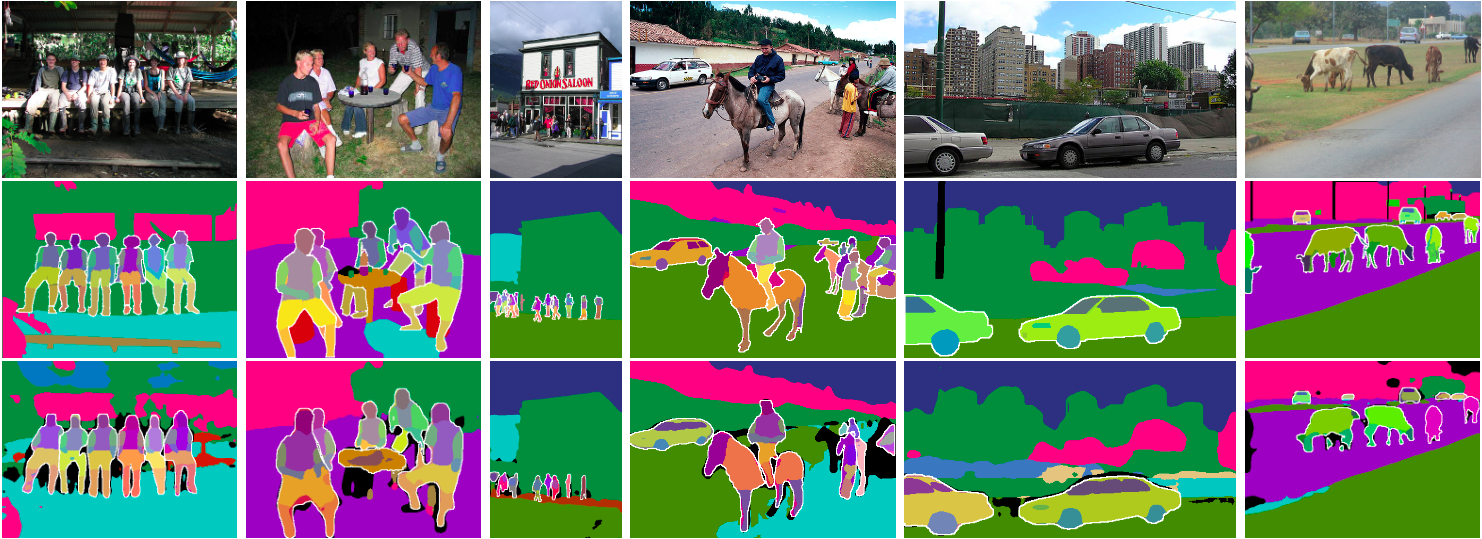
\includegraphics[width=1\linewidth]{recursos/imagens/proposal/part-aware-example.png}
    \label{proposal:proposal:fig:3}
    {\tiny Linhas contendo a imagem de entrada, valor de referencia e segmentação realizada com o método \textit{part-aware}, respectivamente, de cima para baixo.}

    \vspace*{1 cm}
    Fonte: \cite{DeGeus2021}.
\end{figure}

Em resumo, dentre as perspectivas de contribuição deste trabalho, lista-se:

\begin{enumerate}[I]
  \item A utilização da segmentação panóptica hierárquica para a segmentação de componentes visuais na área odontológica;
  \item A disponibilização do código de maneira \textit{open source} com a finalidade de dar suporte aos trabalhos na área de \textit{part-aware panoptica segmentation}.
  \item A avaliação e adaptação (caso necessário) de uma ferramenta que auxilie a anotação de imagens com técnicas de segmentação;
  \item A aplicação da técnica \textit{block-based pca} na camada de \textit{pooling} dos modelos base para a segmentação panóptica.
\end{enumerate}

As demais seções desse capítulo estão organizadas de seguinte modo que a Seção \ref{proposal:matmet} descreve sobre os materiais e métodos utilizados nos experimentos, a Seção \ref{proposal:methodology} descreve a metodologia utilizada em alguns dos experimentos propostos, a Seção \ref{proposal:cron} apresenta um cronograma das atividades neste trabalho, e, finalmente, a Seção \ref{proposal:expres} demonstra alguns resultados esperados no decorrer do andamento do presente trabalho.


\subsection{Materiais e Métodos}
\label{proposal:matmet}
Nesta Seção, serão discorridos os detalhes sobre as tecnologias que serão utilizadas para o desenvolvimento de um modelo de segmentação panóptica que segmenta componentes visuais (Subseção \ref{proposal:tec}), as técnicas e métodos escolhidos para serem utilizados nos experimentos (Subseção \ref{proposal:method}) e, por fim, sobre os conjuntos de dados selecionados para cumprirem com o objetivo da segmentação (Subseção \ref{proposal:dataset}).


\subsubsection{Tecnologias}
\label{proposal:tec}
Dentre as tecnologias planejadas para o desenvolvimento do presente trabalho, vale citar que destaca-se o uso da linguagem de programação interpretada e de alto nível, \textit{Python}, sendo essa uma linguagem vantajosa por ser popularmente conhecida em meio cientifico, com uma ampla comunidade e com  bibliotecas dispostas para facilitar o desenvolvimento de soluções \cite{Millman2011PythonEngineers}.

Já em relação às bibliotecas planejadas ao projeto, destacam-se aquelas cujo desenvolvimento é amplamente utilizado para o auxilio de projetos de visão computacional, aprendizado de máquina e redes neurais, das quais cita-se: \textit{PyTorch}, \textit{Keras}, \textit{TensorFlow}, \textit{OpenCV}, \textit{Numpy}, \textit{Pandas}, entre outras, dando destaque para a biblioteca \textit{Detectron2} \cite{detectron2} que já possui algumas funções especializadas para o trabalho com segmentações, incluindo redes de segmentação panóptica.

Por fim, em relação aos métodos desenvolvido para cumprir com os objetivos do presente trabalho, no que lhes concerne, de realizar a segmentação de componentes visuais, declara-se que serão disponibilizado de modo \textit{Open Source} por meio do \textit{Github} do autor\footnote{Perfil \textit{Github} do autor – \url{https://github.com/Lucs1590}}, segundo os preceitos a licença Apache v2.0 \cite{Licenses}, com o intuito de contribuir com o crescimento de futuros pesquisadores, além de possibilitar futuras melhorias da aréa de segmentação com uso de segmentação hierárquica.


\subsubsection{Métodos}
\label{proposal:method}
Dentre os métodos disponíveis para realizar a tarefa de segmentação panóptica de componentes visuais, destaca-se que serão realizados testes a partir dos modelos disponibilizados pela biblioteca \textit{Detectron2} \cite{detectron2}, seguindo também a formatação inicial proposta por Kirillov \textit{et al.} \cite{Kirillov2019a}, a qual era composta por um modelo de Mask R-CNN (Seção \ref{instance:mask}) para realizar a parte de segmentação de instâncias e o modelo de FCN (Seção \ref{semantic:FCN}) para realizar a segmentação de semântica.

Todavia, haja vista o resultado esperado nesse trabalho, vide a Seção \ref{proposal:expres}, para as tarefas de segmentação panóptica com o uso de partes, diferente das abordagens demonstradas na Figura \ref{proposal:method:fig:1}, necessita também de uma parte voltada para a segmentação das partes de algo classificado como \textit{thing} ou \textit{stuff}, como demonstrado na Figura \ref{proposal:method:fig:2}, desse modo também será testada a estrutura desenhada por de Geus \textit{et al.} \cite{DeGeus2021} a qual é composta por um modelo de segmentação panóptica (DLv3-ResNeSt269 \& DetectoRS) juntamente com um modelo responsável por realizar uma segmentação de partes (BSANet).

\begin{figure}[H]
    \centering
    \caption{Metodologias de rede para segmentação panóptica.}
    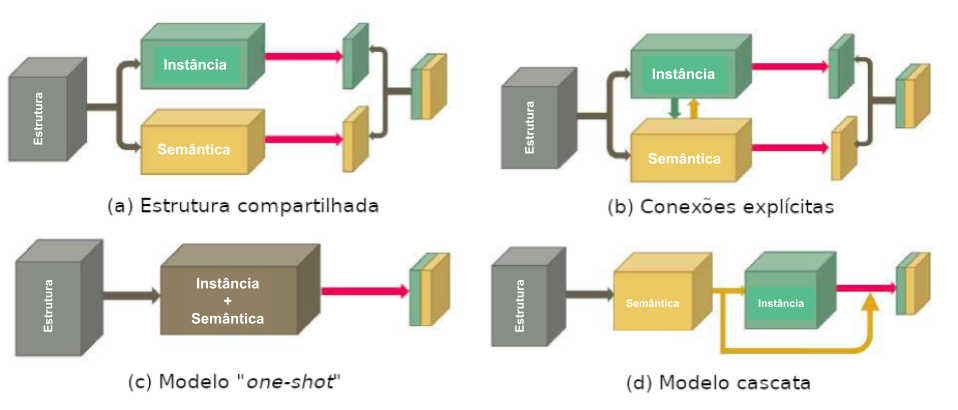
\includegraphics[width=1\textwidth]{recursos/imagens/proposal/model_methodologies.png}
    \label{proposal:method:fig:1}

    \vspace*{1 cm}
    Fonte: retirado e adaptado de \cite{Elharrouss2021}.
\end{figure}

\begin{figure}[H]
    \centering
    \caption{Estrutura exemplificando metodologia para segmentação \textit{Part-Aware}.}
    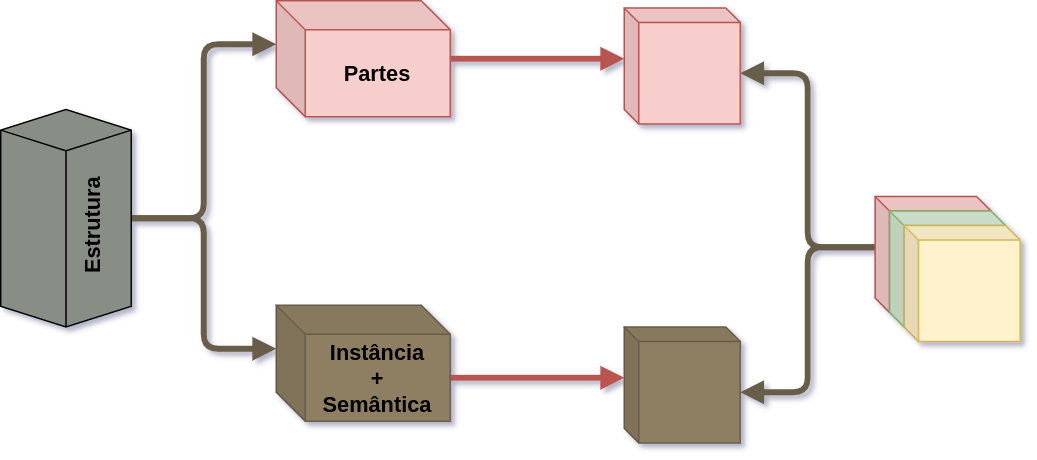
\includegraphics[width=4in]{recursos/imagens/proposal/estrutura.png}
    \label{proposal:method:fig:2}

    \vspace*{1 cm}
    Fonte: do próprio autor.
\end{figure}


\subsubsection{Conjuntos de Dados}
\label{proposal:dataset}
Em relação ao conjunto de dados, por esse trabalho fazer uso da segmentação \textit{Part-Aware Panoptic Segmentation} proposta em \cite{DeGeus2021}, sendo que esta é uma nova abordagem, vale dizer que a quantidade de conjuntos de dados ainda é escassa, principalmente quando se trata de trabalhos voltados para uma área em específico, como a odontológica.

Todavia, no presente trabalho serão utilizados tanto conjuntos de dados que são mais generalistas, mas são voltados para a segmentação panóptica, quanto conjuntos de dados voltados para a parte odontológica, os quais precisarão ser anotados de modo a estarem adaptados para o seu uso em bases de treino e teste.

Quanto aos conjuntos de dados mais generalistas vale dizer que há algumas estratégias e justificativas para o seu uso, as quais serão descritas na Subseção \ref{proposal:transf}, entretanto, dentre os conjuntos de dados escolhidos, destacam-se PASCAL \textit{Panoptic Parts} e \textit{Cityscapes Panoptic Parts}, sendo que os estes foram desenvolvidos pelos autores que abrolharam a segmentação panóptica com uso da técnica \textit{Part-Aware} \cite{DeGeus2021}.

O conteúdo dos conjuntos PASCAL \textit{Panoptic Parts} e \textit{Cityscapes Panoptic Parts} foram criados a partir de dos conjuntos de dados \cite{everingham2010pascal} e \cite{Cordts2016}, sendo que o conteúdo do primeiro está voltado para pessoas, animais, veículos e cenas em locais fechados, quando o segundo conta com cenas de cidades, respectivamente, os quais são exemplificados na Figura \ref{proposal:dataset:fig:1}.

\begin{figure}[H]
   \caption{Imagens originais e anotadas dos \textit{datasets} para \textit{Part-Aware Panoptic Segmentation}.}
   \centering
   \label{proposal:dataset:fig:1}
    \begin{subfigure}[t]{0.45\textwidth}
        \centering
        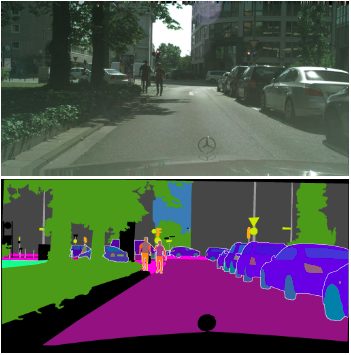
\includegraphics[height=2.5in]{recursos/imagens/proposal/city.png}
        \caption{Imagem original e anotada do \textit{Cityscapes Panoptic Parts}, respectivamente.}
        \label{proposal:dataset:fig:1.1}
    \end{subfigure}%
    ~ 
    \begin{subfigure}[t]{0.45\textwidth}
        \centering
        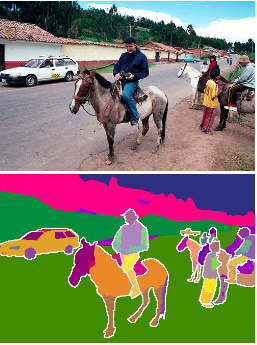
\includegraphics[height=2.5in]{recursos/imagens/proposal/pascal.png}
        \caption{Imagem original e anotada do PASCAL \textit{Panoptic Parts}, respectivamente.}
        \label{proposal:dataset:fig:1.2}
    \end{subfigure}%

    \vspace*{1 cm}
    Fonte: retirado e adaptado de \cite{Lin2016}.
\end{figure}


Os conjuntos criados, os quais contemplam segmentação \textit{Part-Aware}, quando relacionado ao \textit{Cityscape Panoptic Parts}, vale dizer que este possui 2975 imagens para treino e 500 para validação, totalizando em 3475 imagens dispostas em resolução de 1024×2048. Por sua vez, o PASCAL \textit{Panoptic Parts} possui 4998 imagens para treino e  5105 imagens para validação, as quais estão em resoluções de 387×470, totalizando à disposição de 10103 imagens.

Por fim, ainda há a disposição do conjunto de dados PartNet \cite{mo2019}, sendo que este abrange a anotação de 573585 partes de instancias, realizando a cobertura de 24 categorias de objetos, as quais também podem ser úteis para agregar ao projeto.

Quanto aos conjuntos de dados citados anteriormente que estarão dispostos para o meio odontológico, vale citar que esses não possuem uma anotação com classes de partes, as quais se fazem \textit{mister} para a aplicação panóptica com uso de \textit{Part-Aware}, todavia vale destacar que foi estabelecido uma parceria com a Faculdade de Odontologia de Araraquara - UNESP, a qual terá com líder o Prof. Dr. Osmir Batista de Oliveira Júnior, de modo que estudantes e especialistas da área realizem as anotações, bem como a disponibilização, de algumas imagens de fotografias odontológicas, de modo a contribuírem para o projeto.

Além das fotografias cedidas pela parceria estabelecida, vale destacar que alguns conjuntos de dados serão utilizados com o intuito de agregar em volume de imagens, dos quais, cita-se o conjunto de dados desenvolvido por You \textit{et al.} \cite{You2020}, o qual possui 886 anotadas, o conjunto desenvolvido por Hyttinen \textit{et al.} \cite{Hyttinen2020}, com 316 imagens, sendo que 215 desssas imagens possuem uma anotação inicial e, por fim, o conjunto de dados disponível no \textit{website} da Dental Care\footnote{\textit{Website Dental Care} – \url{https://www.dentalcare.com/en-us/research/media-library}}, o qual cede 839 imagens odontológicas como cortesia para estudos e desenvolvimento científico. O objetivo é que todas essas 1370 imagens sejam agregadas à \textit{pipeline} de anotação de modo a se tornarem úteis para a construção do modelo proposto no presente trabalho.

\subsection{Metodologia}
\label{proposal:methodology}
Nesta Seção, será descrito quanto à metodologia adotada para os experimentos a serem realizados, de modo a conquistar os objetivos propostos no presente trabalho. Na Subseção \ref{proposal:transf} será detalhado sobre o processos de transferência de aprendizado a ser realizado no conjunto de dados, na Subseção \ref{proposal:pcapooling} se discorrerá sobre o processo de alteração na camada de \textit{pooling} dos modelos e, finalmente, na Subseção \ref{proposal:avaliation} será descrito o método de avaliação escolhido para a submissão dos modelos.

\subsubsection{Transferência de Aprendizado}
\label{proposal:transf}
Tendo em vista que os conjuntos de dados na área odontológica preparados para a aplicação de segmentação panóptica com o uso da técnica \textit{Part-Aware} são inexistentes e que temos alguns conjuntos de dados que suportam os requisitos dessa técnica, justifica-se o uso de técnicas de transferência de aprendizado \cite{Weiss2016}, mesmo em casos de espaços de características heterogêneos.

A técnica de transferência de aprendizado foi inspirada em casos do mundo real, onde um panorama sobre determinado assunto tende a trazer mais eficacia para o aprendizado de novos assuntos \cite{Pan2010}, mas também para casos em que há uma pequena quantidade de amostras disponíveis em um conjunto de dados alvo para o treinamento de uma rede \cite{Weiss2016}, ocasionando em problemas, haja vista que redes de aprendizado profundo contam de uma grande quantidade de dados para ter bom desempenho \cite{Goodfellow2016}

Sendo assim, por esse projeto se enquadrar no segundo caso citado dentro do paragrafo anterior, onde a quantidade de amostras do conjunto de dados para realizar a fase de treinamento é pequena, a técnica de transferência de aprendizado será adotada, utilizando amostras dos conjuntos de dados PASCAL \textit{Panoptic Parts}, \textit{Cityscapes Panoptic Parts} e PartsNet para o treinamento da rede, até dado momento e, depois, submetendo a mesma rede no conjunto de dados odontológico que será anotado em conjunto com a parceria realizada.


\subsubsection{Alteração na Camada de \textit{Pooling}}
\label{proposal:pcapooling}
Como explicado na Subseção \ref{deep:pooling}, a adaptação dos modelos de \textit{pooling} é crescente, sendo que essas modificações são motivadas pelos problemas a serem resolvidos, sendo assim, quando se trata de segmentações modernas, duas abordagens ganham destaque como técnicas de \textit{pooling}, sendo elas: \textit{Atrous Spatial Pyramid Pooling} (ASPP) \cite{Chen2018} e \textit{Pyramid Pooling} \cite{Zhao2017}.

Basicamente, a abordagem relacionada ao modulo de ASPP está atrelada às segmentações semânticas \cite{Mohan2020}, sendo que este módulo tem como sua principal vantagem a captura de objetos e contexto úteis da imagem em várias escalas diferentes, haja vista que seu comportamento está atrelado à re-amostragem com diversas taxas de convolução para cada \textit{kernel}, possibilitando, assim, a sondagem de um mapa de características, antes mesmo do processo de convolução, com vários campos de visão \cite{Chen2018}.

Já quando se trata do módulo de \textit{Pyramid Pooling}, vale dizer que este está atrelado à dimensão das características, tendo como principal motivação provar ser um \textit{pooling} de contexto global antes de realizar sua representação \cite{Zhao2017}. Todavia, quando se trata desse modelo de \textit{pooling}, vale dizer que a sua maior vantagem está relacionada à flexibilidade que é cedida às entradas das redes, de modo que torna-se possível realizar entradas com tamanhos variados.

Entretanto, vale citar que no presente trabalho, além da escolha dos modelos acima listados, também será realizado um experimento com a aplicação da técnica de \textit{Block-Based Principal Component Analysis} (ou BPCA) nas camadas de \textit{pooling} dos modelos base para a realização da segmentação panóptica. Esse módulo de \textit{pooling}, desenvolvidos por Salvadeo \textit{et al.} \cite{Salvadeo2011} que se provou satisfatório para aplicações relacionado ao reconhecimento de faces, realiza a aplicação do método \textit{Principal Component Analysis} (PCA) nos blocos que divide uma imagem original, de modo a manter as estruturas espacias da imagem original, sendo assim, para o presente trabalho, tem-se a espectativa de adicionar esse método na camada de \textit{pooling} o modelo base, tendo uma  redução de dimensionalidade e mantendo as estruturas originais da entrada em questão, o que normalmente é perdido quando se aplica uma estratégia de \textit{pooling} em escala global (como representado na Figura \ref{deep:fig:7}).


\subsubsection{Avaliação}
\label{proposal:avaliation}
O método de avaliação escolhido seguiu no mesmo caminho do artigo tomado como referência para realizar a segmentação \textit{Part-Aware Panoptic Segmentation} \cite{DeGeus2021}, que, no que lhe concerne, teve como base o artigo pioneiro de segmentação panóptica \cite{Kirillov2019a}, que aplica a métrica PQ (Equação \ref{panoptic:eq:2}), realizando uma sucinta adaptação que possibilita metrificar as partes das segmentações panópticas visto que é aplicado para cada uma das classes ($l$) presentes na cena, sendo elas \textit{thing} ou \textit{stuff}. Através da equação \ref{proposal:avaliation:eq:1} é possível entender a métrica de avaliação \textit{Part-PQ}, a qual fora escolhida para avaliação.

\begin{equation}
\label{proposal:avaliation:eq:1}
    PartPQ = \frac{\sum _{(p,g) \in VP} IoU_p(p,g)}{|VP|+ \frac{1}{2}|FP| + \frac{1}{2}|FN|}.
\end{equation}

Em relação à Equação \ref{proposal:avaliation:eq:1}, destaca-se ainda que a segmentação das partes dentro de um segmento é capturada principalmente por meio do termo $IoU_p(p,g)$, sendo que no termo é aplicado um condicional com o intuito de deixar a classe segmentada com parte ($\mathcal{L}^{parts}$) e sem partes ($\mathcal{L}^{no-parts}$) dentro das mesmas condições, ou seja, para as classes com partes presentes, aplica-se a métrica de $mIoU$ para cada pixel de parte dentro de um segmento, enquanto para segmentações sem partes, aplica-se a $IoU$ que comumente é utilizada na métrica PQ (Equação \ref{panoptic:eq:2}). O condicional supracitado da-se por meio da seguinte expressão:

\begin{equation}
\label{proposal:avaliation:eq:2}
    IoU_p(p,g)= \left\{\begin{matrix}
        mIoU_{part}(p,g), & l \in \mathcal{L}^{parts}    & \\ 
        IOU_{ins}(p,g),        & l \in \mathcal{L}^{no-parts} & 
    \end{matrix}\right.
\end{equation}

Por fim, após a aplicação de PartPQ em todas as classes, calcula-se a média entre avaliações realizadas, de modo que é possível avaliar o desempenho do modelo em toda a cena e demonstrou resultados consideráveis quando comparado à métrica original \cite{DeGeus2021}.


\subsection{Revisão de Literatura}
\label{proposal:revision}
Em meio a vários estilos de revisão, vale dizer que a revisão sistemática é amplamente difundida em meio cientifico, destacando-se em pesquisas de âmbito clínico e médico e garantindo menos viés, maior confiabilidade e um resumo de forma crítica dos trabalhos científicos \cite{barbosa2019}. Sendo assim, no presente trabalho, foi realizado uma revisão, bem como buscas baseadas nos artigos \cite{barbosa2019} e \cite{liberati2009}, de modo que se inspirou nas recomendações dos mesmos, salvo os casos relacionados a questões de aplicações clínicas.

Em relação às revisões, foram realizadas duas, de modo a abranger tanto os artigos técnicos em relação à segmentação panóptica, quanto artigos que servissem de base para a segmentação na área odontológica. A questão a ser tomada como base para esse estudo é: Como modelar \textit{framework} para segmentar imagens de componentes visuais hierarquicamente?

Para a primeira revisão citada, foram procurados todo tipo de estudo publicados a partir do ano de 2019 até o ano presente (2022) com o assunto relacionado a \textit{panoptic segmentation}, de modo a se basear no ano de publicação do artigo pioneiro \cite{Kirillov2019a} no assunto. Foram usados os termos a seguir em diferentes combinações: ``\textit{panoptic segmentation}'', ``\textit{part}'' e ``\textit{part-aware}''. Os idiomas foram restritos à português e inglês.

Os critério de inclusão baseou-se em artigos que possuíssem a citação da técnica de segmentação \textit{part-aware} de modo a contribuir com uma segmentação hierárquica dos componentes que compunham a cena. Já em relação aos critérios de exclusão destaca-se artigos com descrição inadequada em relação ao interesse dessa revisão, quando o artigo era especifico para uma determinada aplicação que não condizia com o tema (como carros autônomos) e quando o estudo estava duplicado entre as ferramentas de busca.

Sendo assim, os indicadores referentes as pesquisas realizadas sobre esse assunto podem ser visualizadas no diagrama abaixo (Figura \ref{proposal:revision:fig:1}).

\begin{figure}[H]
    \centering
    \caption{Diagrama de revisão de estudos em segmentação panóptica.}
    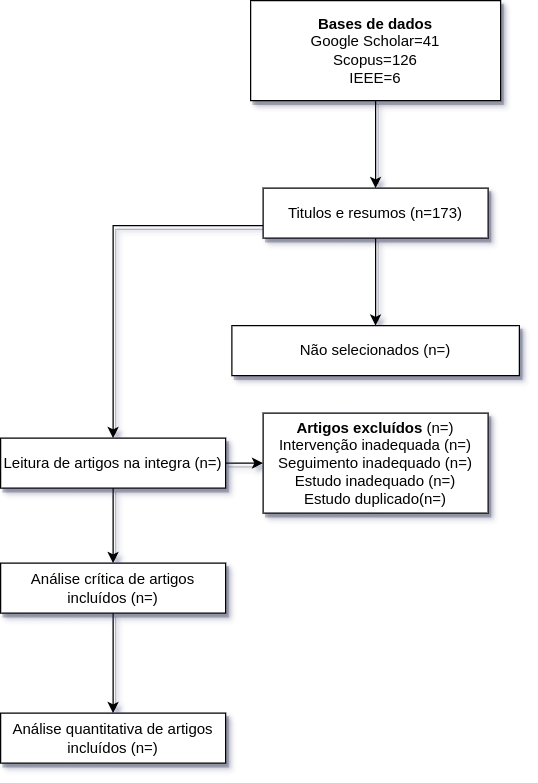
\includegraphics[height=4.5in]{recursos/imagens/proposal/revisao1.png}
    \label{proposal:revision:fig:1}

    \vspace*{1 cm}
    Fonte: do próprio autor.
\end{figure}

\begin{table}[H]
    \centering
    \caption{Trabalhos selecionados a partir da revisão sobre segmentação panóptica.}
    \label{proposal:revision:1}
    \resizebox{\textwidth}{!}{
    \begin{tabular}{l|l|l}
    \textbf{Título}                  &  \textbf{Autores}                 &  \textbf{Referência}  \\ \hline
       &    &    
    \end{tabular}}

    \vspace*{1 cm}
    Fonte: do próprio autor.
\end{table}

Quando se trata da segunda revisão em pauta, a que contempla as segmentações na área odontológica, destaca-se que os estudos procurados também não se limitaram ao tipo, incluindo congressos, artigos de revista, entre outros, além de utilizarem o intervalo dos anos de 2019 a 2022 como métrica, de modo a encontrar segmentações odontológicas que acompanhasse a técnica de segmentação panóptica. Os termos utilizados estão listados a seguir, de modo que foram buscados em diferentes combinações: ``odonto'', ``\textit{dentistry}'', ``\textit{deep learning}'', ``\textit{semantic segmentation}'', ``\textit{instance segmentation}'', ``\textit{panoptic segmentation}'' e ``CNN''. Os idiomas foram restritos à português e inglês.

Quanto aos critérios de inclusão, destaca-se os artigos que abordaram ao menos uma das segmentações modernas, de feitio a estarem alinhados com a proposta do projeto. Quanto aos critérios de exclusão, pode-se dizer que são similares aos da primeira revisão, relatando artigos com descrição inadequada acerca da revisão em questão, estudos duplicados entre as ferramentas de busca e quando o estudo não estava diretamente relacionado aos temas ``segmentação'' e ``odontologia''. Dessa forma, por meio da Figura \ref{proposal:revision:fig:2} é possível visualizar a representação da revisão realizada.

\begin{figure}[H]
    \centering
    \caption{Diagrama de revisão de estudos em segmentação odontológica.}
    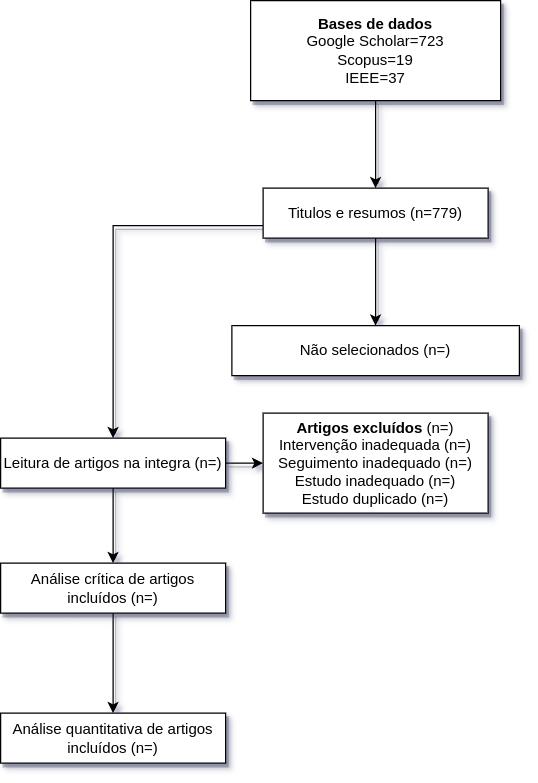
\includegraphics[height=4.5in]{recursos/imagens/proposal/revisao2.png}
    \label{proposal:revision:fig:2}

    \vspace*{1 cm}
    Fonte: do próprio autor.
\end{figure}

\begin{table}[H]
    \centering
    \caption{Trabalhos selecionados a partir da revisão sobre segmentação odontológica.}
    \label{proposal:revision:2}
    \resizebox{\textwidth}{!}{
    \begin{tabular}{l|l|l}
    \textbf{Título}                  &  \textbf{Autores}                 &  \textbf{Referência}  \\ \hline
       &    &    
    \end{tabular}}

    \vspace*{1 cm}
    Fonte: do próprio autor.
\end{table}


\subsection{Cronograma}
\label{proposal:cron}
Com o intuito de listar todas as atividades necessárias para o cumprimento do projeto, bem como definição do período em que as mesmas devem ser realizadas, foram construídas a Tabela \ref{proposal:cron:table:1} e \ref{proposal:cron:table:2}, almejando realizar no máximo quatro  experimentos simultaneamente, considerando a complexidade, esforço e incerteza envolvida em cada um desses testes. Em relação às submissões é desejado realizar uma para conferência, objetivando  contribuir com os experimentos desenvolvidos na primeira etapa e uma segunda para um periódico com o intuito de contribuir com as descobertas realizadas no experimento IV. Por fim, tem se como objetivo realizar a escrita do trabalho em todo o período do cronograma - salvo o mês planejado para a defesa - sendo que essa atividade ocorrera paralelamente aos demais experimentos e atividades listadas. Por fim, vale lembrar, como citado na Subseção \ref{proposal:dataset}, que o trabalho de anotação das imagens ocorrerá em parceria com estudantes e a equipe coordenada pelo Prof. Dr. Osmir Batista de Oliveira Júnior. 

\definecolor{midgray}{gray}{.5}

\begin{table}[H]
    \centering
    \caption{Atividades a serem desenvolvidas.}
    \label{proposal:cron:table:1}
    \resizebox{\textwidth}{!}{
        \begin{tabular}{l|l}
            \textbf{Índice} & \textbf{Descrição}                                                                                                             \\ \hline
            I - 1           & Obtenção e anotação de imagens odontológicas para o treinamento e teste da rede.                                               \\
            I - 2           & Aplicação da biblioteca \textit{Detectron2} para realização de segmentação panóptica.                                          \\
            I - 3           & Modelagem da rede com o uso de \textit{part-aware panoptic segmentation}, segundo sugerido por \cite{DeGeus2021}.              \\
            I - 4           & Submissão de testes na rede modelada, com o intuito de saber como a rede tem performado.                                       \\
            II - 1          & Avaliar e adaptar (caso necessário) uma ferramenta que auxilie a anotação de imagens;                                          \\
            III - 1         & Desenvolvimento de biblioteca \textit{open source} com métodos que auxiliam a segmentação hierárquica de componentes visuais.  \\
            IV - 1          & Transferência de aprendizado entre os conjuntos de dados disponíveis e conjunto de dado anotado.                               \\
            IV - 2          & Modificação da arquitetura base para aplicação de \textit{block-based PCA} na camada de \textit{pooling};                      \\
            V - I           & Desenvolvimento de métodos de visualização da informação para comparar os conjuntos de dados e as métricas das redes.          \\
            V - II          & Comparação de rede de segmentação panóptica com a rede desenvolvida.                                                 
        \end{tabular}
    }

    \vspace*{1 cm}
    Fonte: do próprio autor.
\end{table}


\begin{table}[ht]
    \centering
    \caption{Cronograma de atividades.}
    \label{proposal:cron:table:2}
        \begin{tabular}{|c|c|c|c|c|c|c|l|l|} 
            \hline
                                    & \multicolumn{8}{c|}{2022}                        \\ 
            \hline
            \textbf{Macroatividades}        & FEV & MAR & ABR & MAI & JUN & JUL & AGO & SET  \\ 
            \hline
            Experimento I                   & \cellcolor{midgray} & \cellcolor{midgray} & \cellcolor{midgray} &     &     &     &     &      \\ 
            \hline
            Experimento II                 &     & \cellcolor{midgray} & \cellcolor{midgray} &     &     &     &     &      \\ 
            \hline
            Experimento III                  &     &     &     & \cellcolor{midgray} & \cellcolor{midgray} & \cellcolor{midgray} &     &  \\ 
            \hline
            Experimento IV                  &     &     &     & \cellcolor{midgray} & \cellcolor{midgray} &     &     &      \\ 
            \hline
            Experimento V                   &     &     &     &     &     & \cellcolor{midgray} &     &      \\ 
            \hline
            Escrita da dissertação          & \cellcolor{midgray} & \cellcolor{midgray} & \cellcolor{midgray} & \cellcolor{midgray} & \cellcolor{midgray} & \cellcolor{midgray} & \cellcolor{midgray} &  \\ 
            \hline
            Submissão para conferência      &     &     &     & \cellcolor{midgray} &     &     &     &      \\ 
            \hline
            Submissão para periódico        &     &     &     &     &     &     & \cellcolor{midgray} &      \\ 
            \hline
            Defesa                          &     &     &     &     &     &     &     & \cellcolor{midgray} \\
            \hline
        \end{tabular}
    
    \vspace*{1 cm}
    Fonte: do próprio autor.
\end{table}


\subsection{Resultados Esperados}
\label{proposal:expres}
Tendo em vista as quatro principais propostas que estão resumidas no Capítulo \ref{proposal:proposal}, vale dizer que para cada uma delas há a esperança de colher resultados.

No que diz respeito a aplicação de segmentação de componentes visuais na área odontológica, destaca-se que esse é o ponto que coloca o desenvolvimento de frente a problemas reais, com o objetivo de obter a maior descrição de cena possível no contexto odontológico, assim auxiliando profissionais da área na evidenciação de caracteristicas da boca. Essa proposta foi iniciada a partir do estudo realizado por \cite{DeGeus2021} que busca, por meio do \textit{Part-Awere Panoptic Segmentation}, trazer uma visão mais holística das cenas. Sendo assim, com a meta de esclarecer visualmente esse resultado esperado, a expectativa é que por meio da entrada de uma imagem, como a representada pela Figura \ref{proposal:expres:fig:4}, tenha-se como saída da rede uma outra imagem, como a representada pela Figura \ref{proposal:expres:fig:5}.

\begin{figure}[H]
    \centering
    \caption{Exemplo de imagem de entrada para a rede a ser desenvolvida.}
    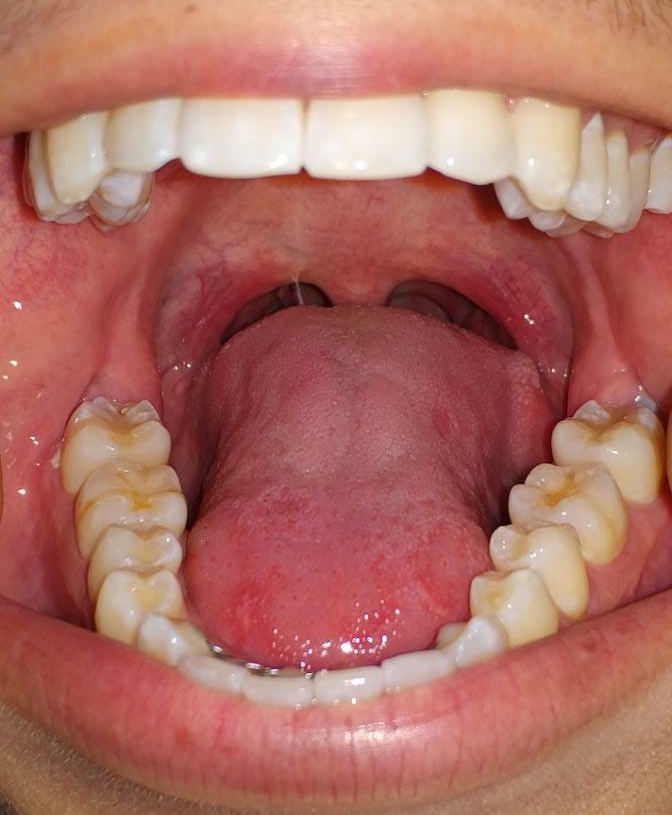
\includegraphics[height=4.3in]{recursos/imagens/proposal/boca.png}
    \label{proposal:expres:fig:4}

    \vspace*{1 cm}
    Fonte: do próprio autor.
\end{figure}

\begin{figure}[H]
    \centering
    \caption{Exemplo de imagem de saída esperada pela rede a ser desenvolvida.}
    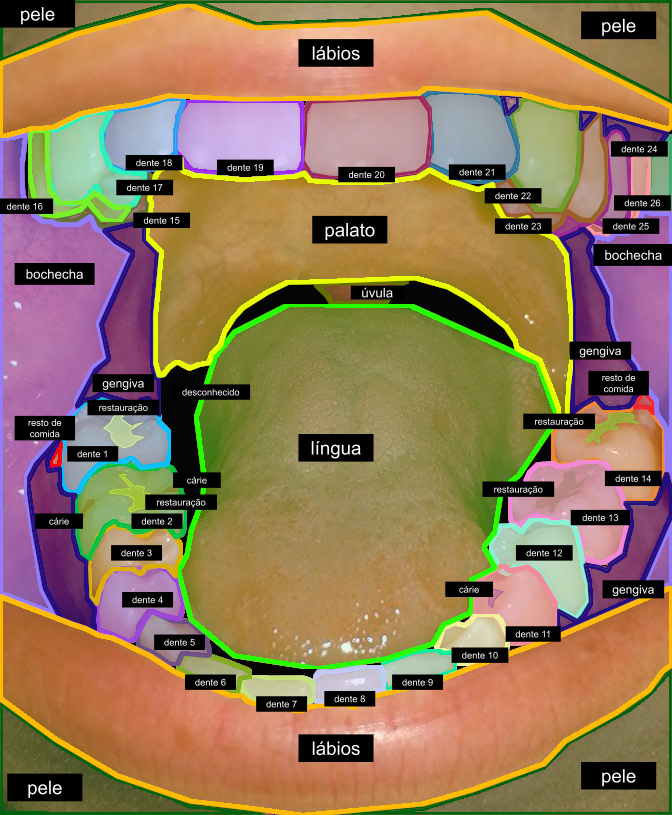
\includegraphics[height=4.3in]{recursos/imagens/proposal/boca_segmentada_v2.png}
    \label{proposal:expres:fig:5}

    \vspace*{1 cm}
    Fonte: do próprio autor.
\end{figure}

Tendo observado e considerando as figuras de entrada e saída, respectivamente, Figura \ref{proposal:expres:fig:4}
 e \ref{proposal:expres:fig:5}, pode-se dizer que uma descrição de cena que se encaixa na representação da Figura \ref{proposal:expres:fig:5}, dadas às segmentações pode ser: Fotografia de uma boca contendo ``pele'', ``lábios'', ``bochechas'', ``gengivas'', ``palato mole'', ``língua'' e ``úvula'', como o tipo \textit{stuff}. Além disso, tem-se como parte da ``gengiva'', ``resto de comida''. Já em relação às instâncias (\textit{things}), nessa fotografia, encontram-se ``26 dentes'', sendo que é possível localizar como partes dos dentes 1, 2 e 11, ``cáries'' e como parte dos dentes 1, 2, 13 e 14, ``restaurações''.

Essa descrição de resultado esperado bem como as segmentações exemplificadas só são possíveis por meio de uma segmentação panóptica com uma segmentação voltada para as partes, o que suporta o uso do método estudado em \cite{DeGeus2021}, estabelecendo, assim, uma segmentação hierárquica de componentes visuais.

Caso a técnica de segmentação escolhida fosse a semântica, a contagem de dentes não seria possível. Por outro lado, se a segmentação escolhida fosse a de instâncias, partes como gengivas, comissuras e partes incontáveis seriam ignoradas e, por fim, caso a segmentação escolhida fosse a panóptica, desenvolvida por Kirillov \textit{et al.} \cite{Kirillov2019a}, não seria possível estabelecer uma relação entre as partes das classes, como é exemplificado na Figura \ref{proposal:expres:fig:6}, onde as cáries e a restauração são parte do ``dente 2''.

\begin{figure}[H]
    \centering
    \caption{Exemplo de hierarquia entre componentes visuais.}
    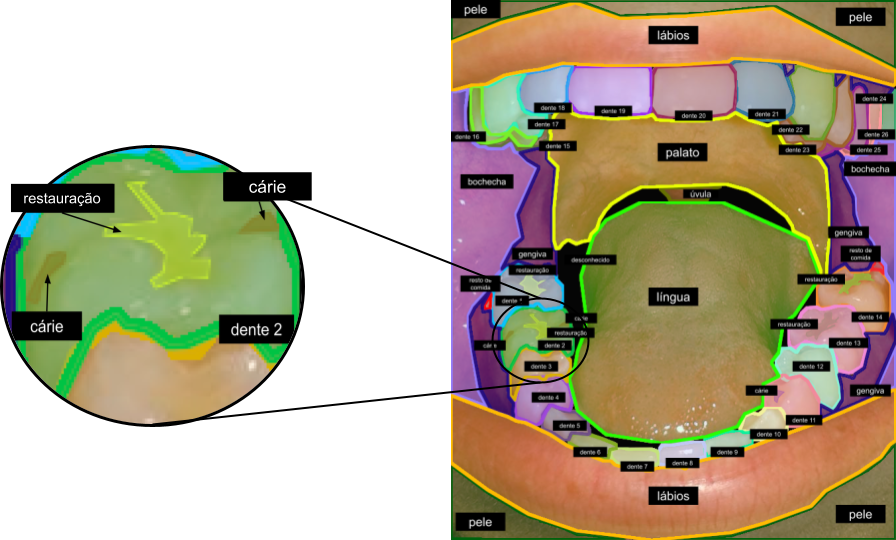
\includegraphics[width=1\textwidth]{recursos/imagens/proposal/segmentada.png}
    \label{proposal:expres:fig:6}

    \vspace*{1 cm}
    Fonte: do próprio autor.
\end{figure}

Em resumo, no presente trabalho, quanto à segmentação hierárquica de componentes visuais espera-se a realização de um \textit{framework} que mapeie fotografias odontológicas, retornando as estruturas da boca e, principalmente, possibilitando a contagem de dentes e a presença de caries.
 
Em relação a contribuição com a publicação dos códigos para a segmentação hierárquica de componentes visuais é esperado que seja desenvolvido uma biblioteca que facilite e colabore com o desenvolvimento de novos métodos de segmentação panóptica com o uso de \textit{part-aware}, além de acelerar o desenvolvimento com os códigos já desenvolvidos no presente trabalho.

Acerca da avaliação e adaptação de uma ferramenta de segmentação para a anotação das imagens, vale dizer que essa é uma tarefa de suma importância, de modo a se tornar escalável a atividade de anotação de imagens para com a parceria estabelecida entre a Faculdade de Odontologia de Araraquara, além de trazer velocidade às fases de treino e teste do modelo a ser desenvolvido. Destarte, quanto ao ponto relatado a expectativa é que no final das análises, uma ferramenta tenha uma análise comparativa entre as ferramentas estudadas e que uma seja determinada para a anotações recorrentes que ocorrerão nesse projeto, além de contar com contribuições para a ferramenta escolhida caso sua implementação não seja suficiente, propondo, assim, auxiliar na segmentação com o uso de segmentação panóptica, técnica que já fora testada para essa atividade em outros estudos \cite{Elharrouss2021, Jasper2020}.

Por fim, com respeito à aplicação da técnica BPCA nas camadas de \textit{pooling} dos modelos base, a esperança é que haja uma redução de dimensionalidade mantendo as estruturas espacias da imagem em questão, trazendo, assim, resultados positivos quanto às métricas de PQ e PartPQ.